% !Mode:: "TeX:UTF-8" 

\setcounter{tocdepth}{1}                % 目录深度——\section
\setcounter{secnumdepth}{0}             % 编码深度——\chapter

\titleformat{\chapter}{\huge}{}{1em}{}

\BiChapter{第三章}{Figures, Tables and Equations}

\BiSection{3.1}{Figures}

\fancyhead[R]{本题3.1由QC.Z完成}

解:

\scalebox{3}{$M_2$采用有二极管连接的NMOS器件:}

%$g_m=\sqrt{2\mu_nC_{ox}\frac{W}{L}I_D}$

$C_{ox}=\frac{\epsilon_{ox}}{T_{ox}}=\frac{3.9 \times 8.854 \times 10^{-12}\frac{F}{m}}{9 \times 10^{-9}m}=3.837 \times 10^{-3}\frac{F}{m^2}$

$V_o=V_{DD}-V_{GS2}$

$V_{GS2}=V_{DD}-V_o$

$V_{DS2}=V_{DD}-V_o$

$V_{TH}=V_{TH0}+\gamma(\sqrt{|2\Phi_F+V_{SB}|}-\sqrt{|2\Phi_F|})$

$I_{D2}=\frac{1}{2}\mu_nC_{ox}(\frac{W}{L})_2(V_{GS2}-V_{TH})^2(1+\lambda_n V_{DS2})$

$V_o=V_{SB}$

$g_{m1}=\sqrt{2\mu_nC_{ox}(\frac{W}{L})_1I_{D1}}$

$g_{m2}=\sqrt{2\mu_nC_{ox}(\frac{W}{L})_2I_{D2}}$

$r_o=r_{o1}=r_{o2}=\frac{1}{\lambda_n I_D}$

$g_{mb2}=\frac{g_{m2}\gamma}{2\sqrt{2\Phi_F+V_{SB}}}$

%$R_{out}=[\frac{1}{g_{m2}+g_{mb2}+(r_{o2})^{-1}}]||r_{o1}$

$R_{out}=\frac{1}{g_{m2}+g_{mb2}+r_{o2}^{-1}}||r_{o1}$

$A_v=-g_{m1}R_{out}$

联立以上各式得$A_v=-1.85$






\scalebox{3}{$M_2$采用有二极管连接的PMOS器件:}

$g_{m2}=\sqrt{2\mu_pC_{ox}(\frac{W}{L})_2I_{D2}}$

$r_{o2}=\frac{1}{\lambda_p I_D}$

%$R_{out}=[\frac{1}{g_{m2}+(r_{o2})^{-1}}]||r_{o1}$

$R_{out}=\frac{1}{g_{m2}+r_{o2}^{-1}}||r_{o1}$

修改以上三式后同理得$A_v=-3.57169656548093=-3.57$














	\color{blue}{
	
	\{
	
	\scalebox{3}{$M_2$采用有二极管连接的NMOS器件:}
	
	$V_{GS2}=V_{DD}-V_o$
	
	$V_{DS2}=V_{DD}-V_o$
	
	$V_{TH}=V_{TH0}+\gamma(\sqrt{|2\Phi_F+V_{SB}|}-\sqrt{|2\Phi_F|})$
	
	$I_{D2}=\frac{1}{2}\mu_nC_{ox}(\frac{W}{L})_2(V_{GS2}-V_{TH})^2(1+\lambda_n V_{DS2})$
	
	将前三式代入第四式
	
	\begin{figure}[H] %H为当前位置,!htb为忽略美学标准,htbp为浮动图形
		\begin{minipage}{\linewidth}
			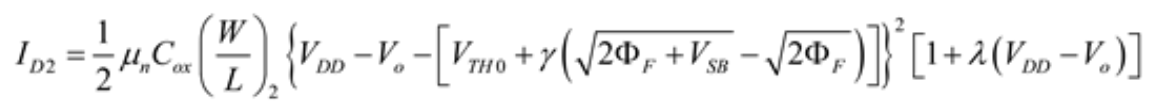
\includegraphics[width=1\linewidth]{3.1-1}
		\end{minipage}
	\end{figure}

	代入$V_o=V_{SB}$
	
		\begin{figure}[H] %H为当前位置,!htb为忽略美学标准,htbp为浮动图形
		\begin{minipage}{\linewidth}
			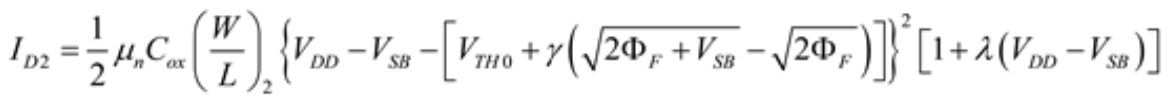
\includegraphics[width=1\linewidth]{3.1-2}
		\end{minipage}
	\end{figure}
	
	\begin{figure}[H] %H为当前位置,!htb为忽略美学标准,htbp为浮动图形
		\begin{minipage}{\linewidth}
			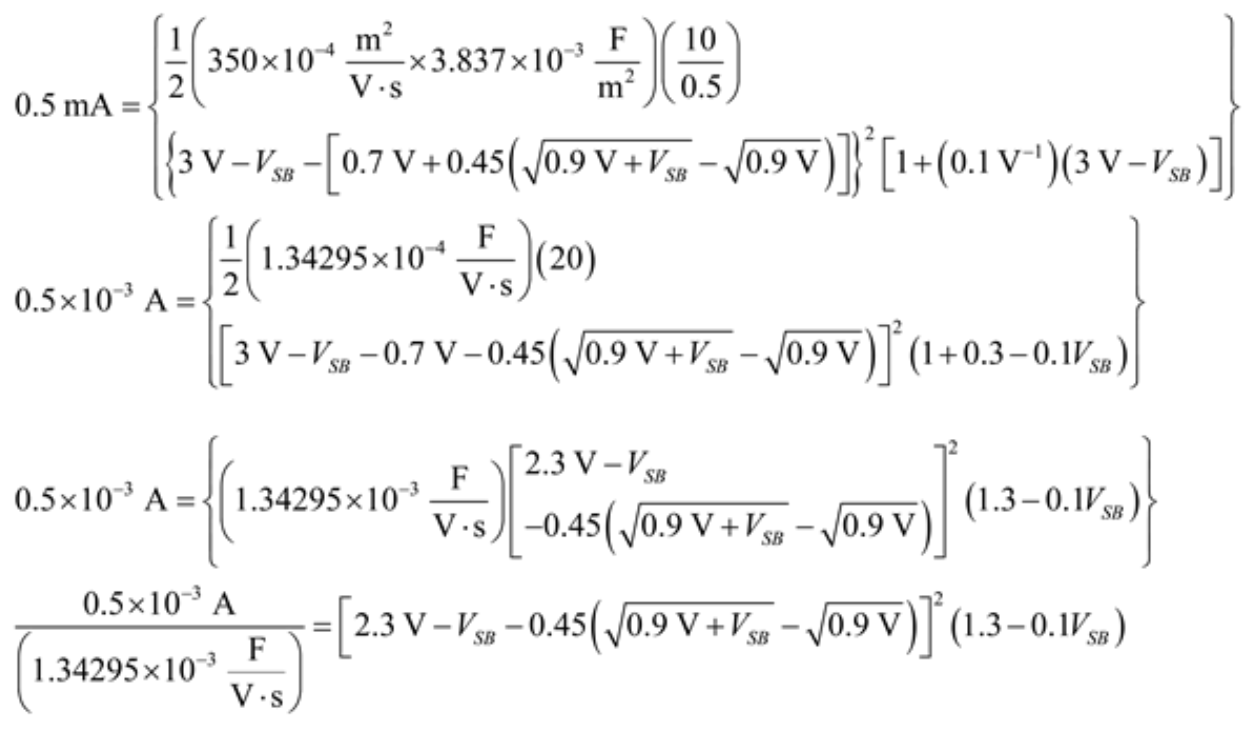
\includegraphics[width=1\linewidth]{3.1-3}
		\end{minipage}
	\end{figure}
	
	\begin{figure}[H] %H为当前位置,!htb为忽略美学标准,htbp为浮动图形
		\begin{minipage}{\linewidth}
			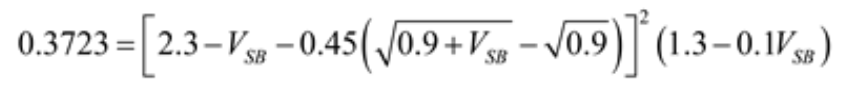
\includegraphics{3.1-4}
		\end{minipage}
	\end{figure}
	
	\begin{figure}[H] %H为当前位置,!htb为忽略美学标准,htbp为浮动图形
		\begin{minipage}{\linewidth}
			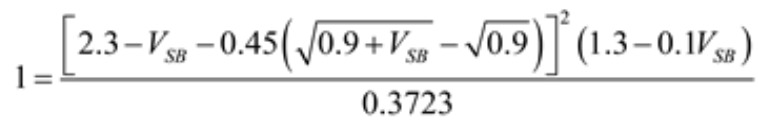
\includegraphics{3.1-5}
		\end{minipage}
	\end{figure}
	
	下面用试错法找$V_{SB}$
	
	\begin{figure}[H] %H为当前位置,!htb为忽略美学标准,htbp为浮动图形
		\begin{minipage}{\linewidth}
			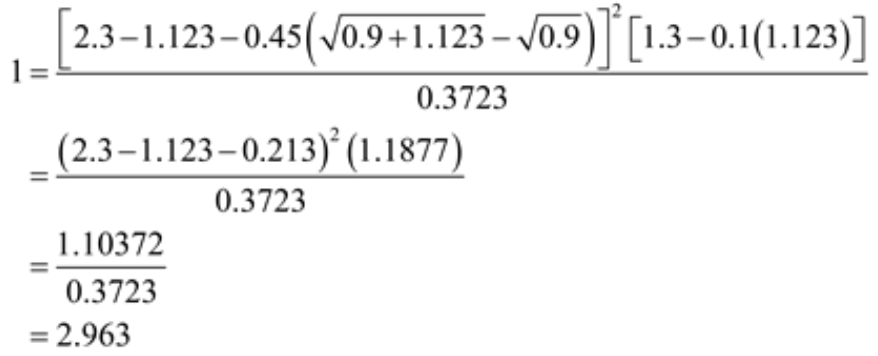
\includegraphics{3.1-6}
		\end{minipage}
	\end{figure}
	
			\begin{figure}[H] %H为当前位置,!htb为忽略美学标准,htbp为浮动图形
		\begin{minipage}{\linewidth}
			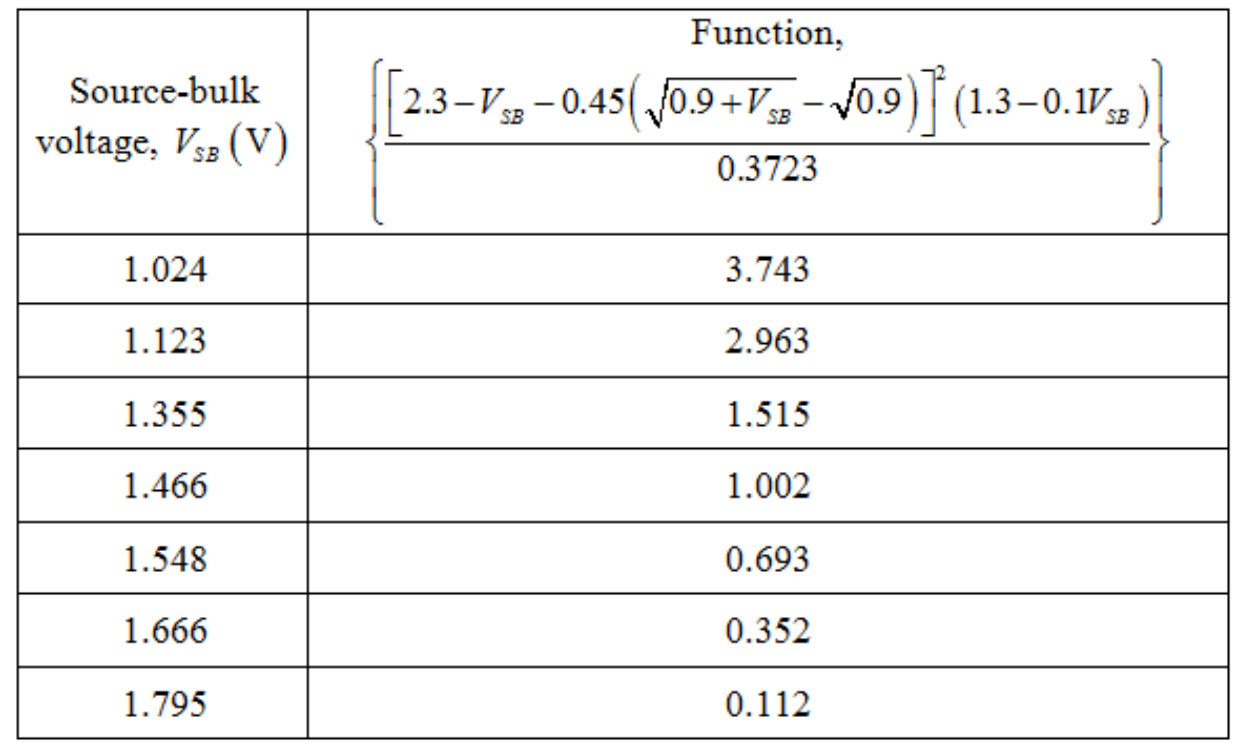
\includegraphics[width=1\linewidth]{3.1-7}
		\end{minipage}
		\caption*{表1} %最终文档中希望显示的图片标题
	\end{figure}
	
	
	
	因此$V_{SB}=1.466V$(这一步用程序会算出三个值,取最小的,认为源衬底即地衬底电压相差不大)
	
	$g_{m1}=\sqrt{2\mu_nC_{ox}(\frac{W}{L})_1I_{D1}}$
	
	\begin{figure}[H] %H为当前位置,!htb为忽略美学标准,htbp为浮动图形
		\begin{minipage}{\linewidth}
			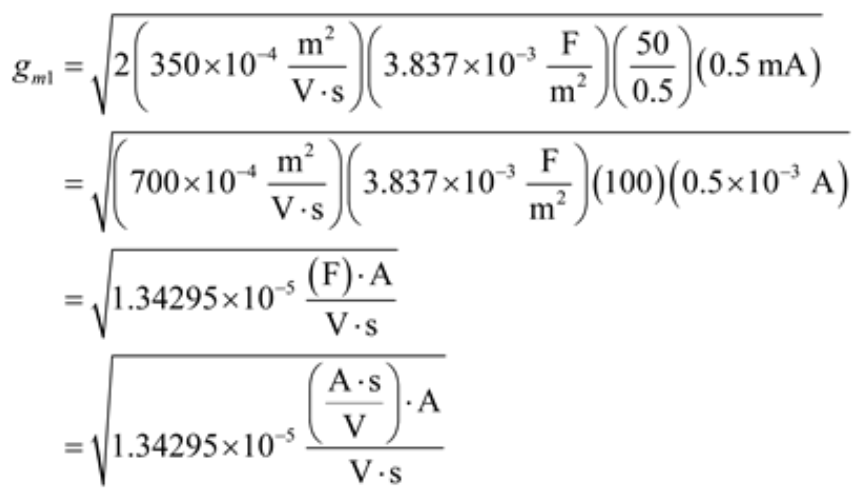
\includegraphics{3.1-8}
		\end{minipage}
	\end{figure}
	
	\begin{figure}[H] %H为当前位置,!htb为忽略美学标准,htbp为浮动图形
		\begin{minipage}{\linewidth}
			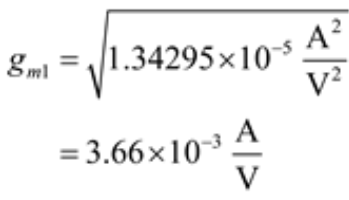
\includegraphics{3.1-9}
		\end{minipage}
	\end{figure}
	
	$g_{m2}=\sqrt{2\mu_nC_{ox}(\frac{W}{L})_2I_{D2}}$
	
	\begin{figure}[H] %H为当前位置,!htb为忽略美学标准,htbp为浮动图形
		\begin{minipage}{\linewidth}
			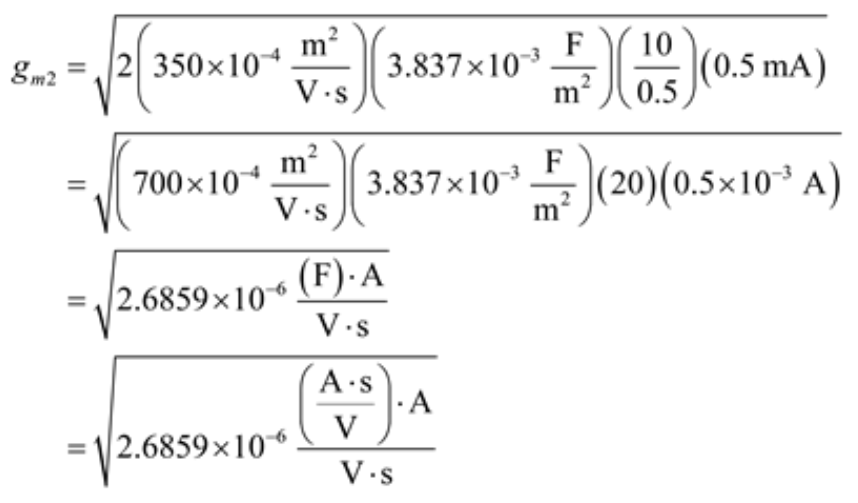
\includegraphics{3.1-10}
		\end{minipage}
	\end{figure}
	
	\begin{figure}[H] %H为当前位置,!htb为忽略美学标准,htbp为浮动图形
		\begin{minipage}{\linewidth}
			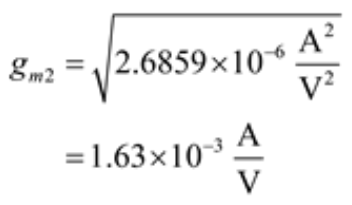
\includegraphics{3.1-11}
		\end{minipage}
	\end{figure}
	
	$r_o=r_{o1}=r_{o2}=\frac{1}{\lambda_n I_D}$
	
	\begin{figure}[H] %H为当前位置,!htb为忽略美学标准,htbp为浮动图形
		\begin{minipage}{\linewidth}
			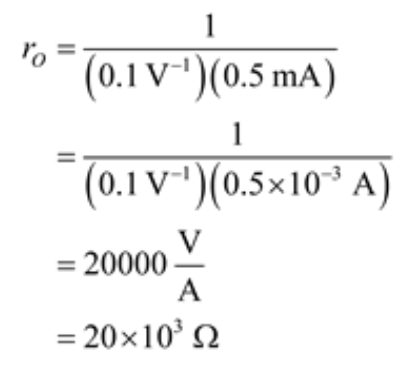
\includegraphics{3.1-12}
		\end{minipage}
	\end{figure}
	
	$g_{mb2}=\frac{g_{m2}\gamma}{2\sqrt{2\Phi_F+V_{SB}}}$
	
	\begin{figure}[H] %H为当前位置,!htb为忽略美学标准,htbp为浮动图形
		\begin{minipage}{\linewidth}
			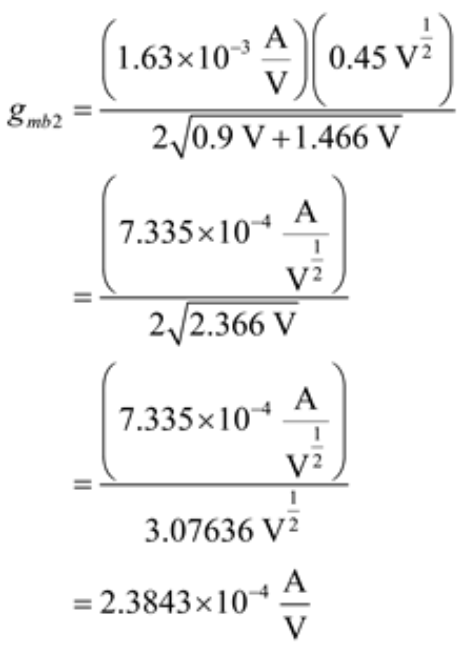
\includegraphics{3.1-13}
		\end{minipage}
	\end{figure}
	
	$R_{out}=\frac{1}{g_{m2}+g_{mb2}+r_{o2}^{-1}}||r_{o1}$
	
	\begin{figure}[H] %H为当前位置,!htb为忽略美学标准,htbp为浮动图形
		\begin{minipage}{\linewidth}
			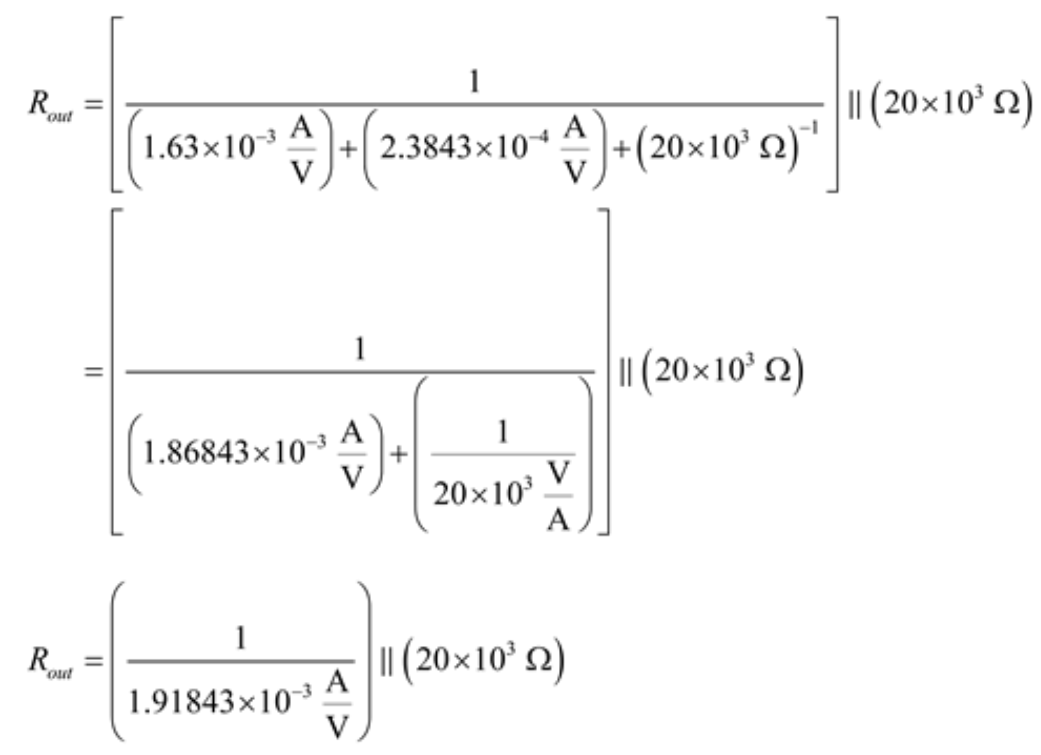
\includegraphics{3.1-14}
		\end{minipage}
	\end{figure}
	
	\begin{figure}[H] %H为当前位置,!htb为忽略美学标准,htbp为浮动图形
		\begin{minipage}{\linewidth}
			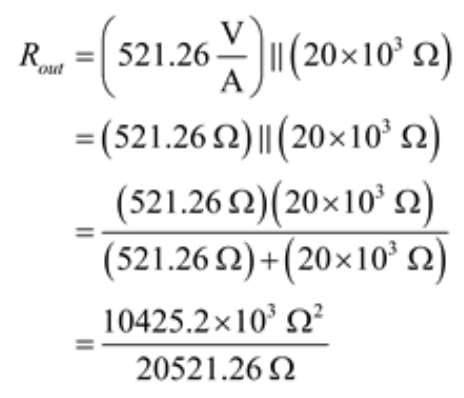
\includegraphics{3.1-15}
		\end{minipage}
	\end{figure}
	
	$R_{out}=508\Omega$
	
	$A_v=-g_{m1}R_{out}$
	
	\begin{figure}[H] %H为当前位置,!htb为忽略美学标准,htbp为浮动图形
		\begin{minipage}{\linewidth}
			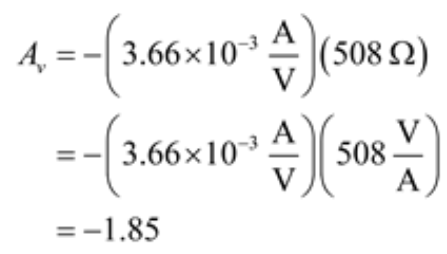
\includegraphics{3.1-16}
		\end{minipage}
	\end{figure}
	
	
	
	
	
	
	
	\}
	
	
	
	
	
	
}









\color{black}{
	
}